
%(BEGIN_QUESTION)
% Copyright 2011, Tony R. Kuphaldt, released under the Creative Commons Attribution License (v 1.0)
% This means you may do almost anything with this work of mine, so long as you give me proper credit

Read selected portions of the Allen-Bradley ``MicroLogix 1000 Programmable Controllers (Bulletin 1761 Controllers)'' user manual (document 1761-6.3, July 1998) and answer the following questions:

\vskip 10pt

Identify the different types of {\it timer} instructions available in the MicroLogix 1000 controller, explaining how each one functions.  How do these types compare with those offered in the Siemens S7-200 PLC?

\vskip 10pt

Identify a practical application for a {\it retentive} timer instruction programmed into a PLC.

\vskip 10pt

How many different options do the Allen-Bradley MicroLogix timer instructions provide for resolution?

\vskip 10pt

How long can one of these timer instructions time up to?  Based on this maximum value, how many bits do you think are used in the register to store a timer instruction's current value?

\vskip 10pt

Sketch a simple ladder-diagram program for an Allen-Bradley MicroLogix 1000 PLC whereby a switch connected to input {\tt I:0/2} causes a timer to increment (count {\it up}) and then turn on an alarm light output {\tt O:0/1} after 5 seconds.  

\vskip 20pt \vbox{\hrule \hbox{\strut \vrule{} {\bf Suggestions for Socratic discussion} \vrule} \hrule}

\begin{itemize}
\item{} If you have access to your own PLC for experimentation, I urge you to write a simple {\it demonstration} program in your PLC allowing you to explore the behavior of these PLC instructions.  The program doesn't have to do anything useful, but merely demonstrate what each instruction does.  First, read the appropriate section in your PLC's manual or instruction reference to identify the proper syntax for that instruction (e.g. which types of data it uses, what address ranges are appropriate), then write the simplest program you can think of to demonstrate that function in isolation.  Download this program to your PLC, then run it and observe how it functions ``live'' by noting the color highlighting in your editing program's display and/or the numerical values manipulated by each instruction.  After ``playing'' with your demonstration program and observing its behavior, write comments for each rung of your program explaining in your own words what each instruction does.
\item{} Some of the addressing examples given in the Allen-Bradley MicroLogix 1000 manual for timer instructions use forward-slash characters ({\tt /}) while other examples use dot characters ({\tt .}) to delimit the last portion of the address.  What do these different characters mean in Allen-Bradley addressing?  For example, what is the different between {\tt T4:0/EN} and {\tt T4:0.ACC}?  Why must the ``EN'' be preceded by a forward slash while the ``ACC'' is preceded by a dot?
\end{itemize}

\underbar{file i00247}
%(END_QUESTION)





%(BEGIN_ANSWER)


%(END_ANSWER)





%(BEGIN_NOTES)

The three Allen-Bradley timer instructions include the On-Delay Timer (TON), Retentive On-Delay Timer (RTO), and Off-Delay Timer (TOF).  Both the TON and RTO timer instructions count time when activated, the difference between them being what happens when their inputs are de-activated: the TON immediately clears while the RTO retains its count value.  The TOF timer instruction counts time when its input is de-activated.

\vskip 10pt

A practical application for a retentive (RTO) timer instruction is one where we must accumulate total time for multiple ``on'' events (e.g. total run-time accumulator for a machine).

\vskip 10pt

Only two resolutions provided: 10 ms and 1 second.

\vskip 10pt

These counters have a maximum count value of 32,767 (15 bit binary number).  This is the positive half of a 16-bit signed integer.

$$\includegraphics[width=15.5cm]{i00247x01.eps}$$


%INDEX% Reading assignment: Allen-Bradley MicroLogix 1000 user manual (timer instructions)

%(END_NOTES)


